\documentclass[a4paper, 12pt]{article}
\usepackage[english]{babel}
\usepackage[a4paper,left=2.5cm, right=2.0cm, top=2.5cm, bottom=2.5cm]{geometry}
\usepackage[utf8]{inputenc}
\usepackage{setspace}
\usepackage{url}
\usepackage{hyperref}
\usepackage{longtable}
\usepackage{lscape}
\usepackage[final]{pdfpages}
\usepackage{graphicx}
\usepackage{colortbl}
\usepackage{multirow}
\usepackage{listings}
\begin{document}
%This file will subsume all of the individual chapters of the project report


%\setstretch{1.50}
\pagestyle{empty}

\begin{center} Project Report \end{center}
\hspace{1cm}
\begin{center} Softwareproject: \end{center}
\begin{center}Spoken Dialog Systems for Elevator Control \end{center}
\begin{center} Universität des Saarlandes \end{center}
\begin{center} Department 4.7 Computational Linguistics and Phonetics \end{center}
\begin{center} Computerlinguistik, B.Sc./M.Sc. \end{center}
\begin{center} Summer term 2015 \end{center} 

\hspace{1cm}
\begin{center}Instructors: Ingmar Steiner, Asad Sayeed, Arif Khan \end{center}

\begin{center} Participants: Anne-Julia Hoffmann, Boyuan Deng, Laura Faust \end{center}


\pagestyle{plain}
\setcounter{page}{1}

%please put in the files you wrote in the corresponding order and space by 
%using \input{filename} so that we can compile the entire project report as one

\section{Dialogue System}

\subsection{ASR}

\subsubsection{Acoustic model}
Training etc.
\subsection{Reverberation recordings in the elevator}

\begin{figure}[h]
\hspace*{3cm}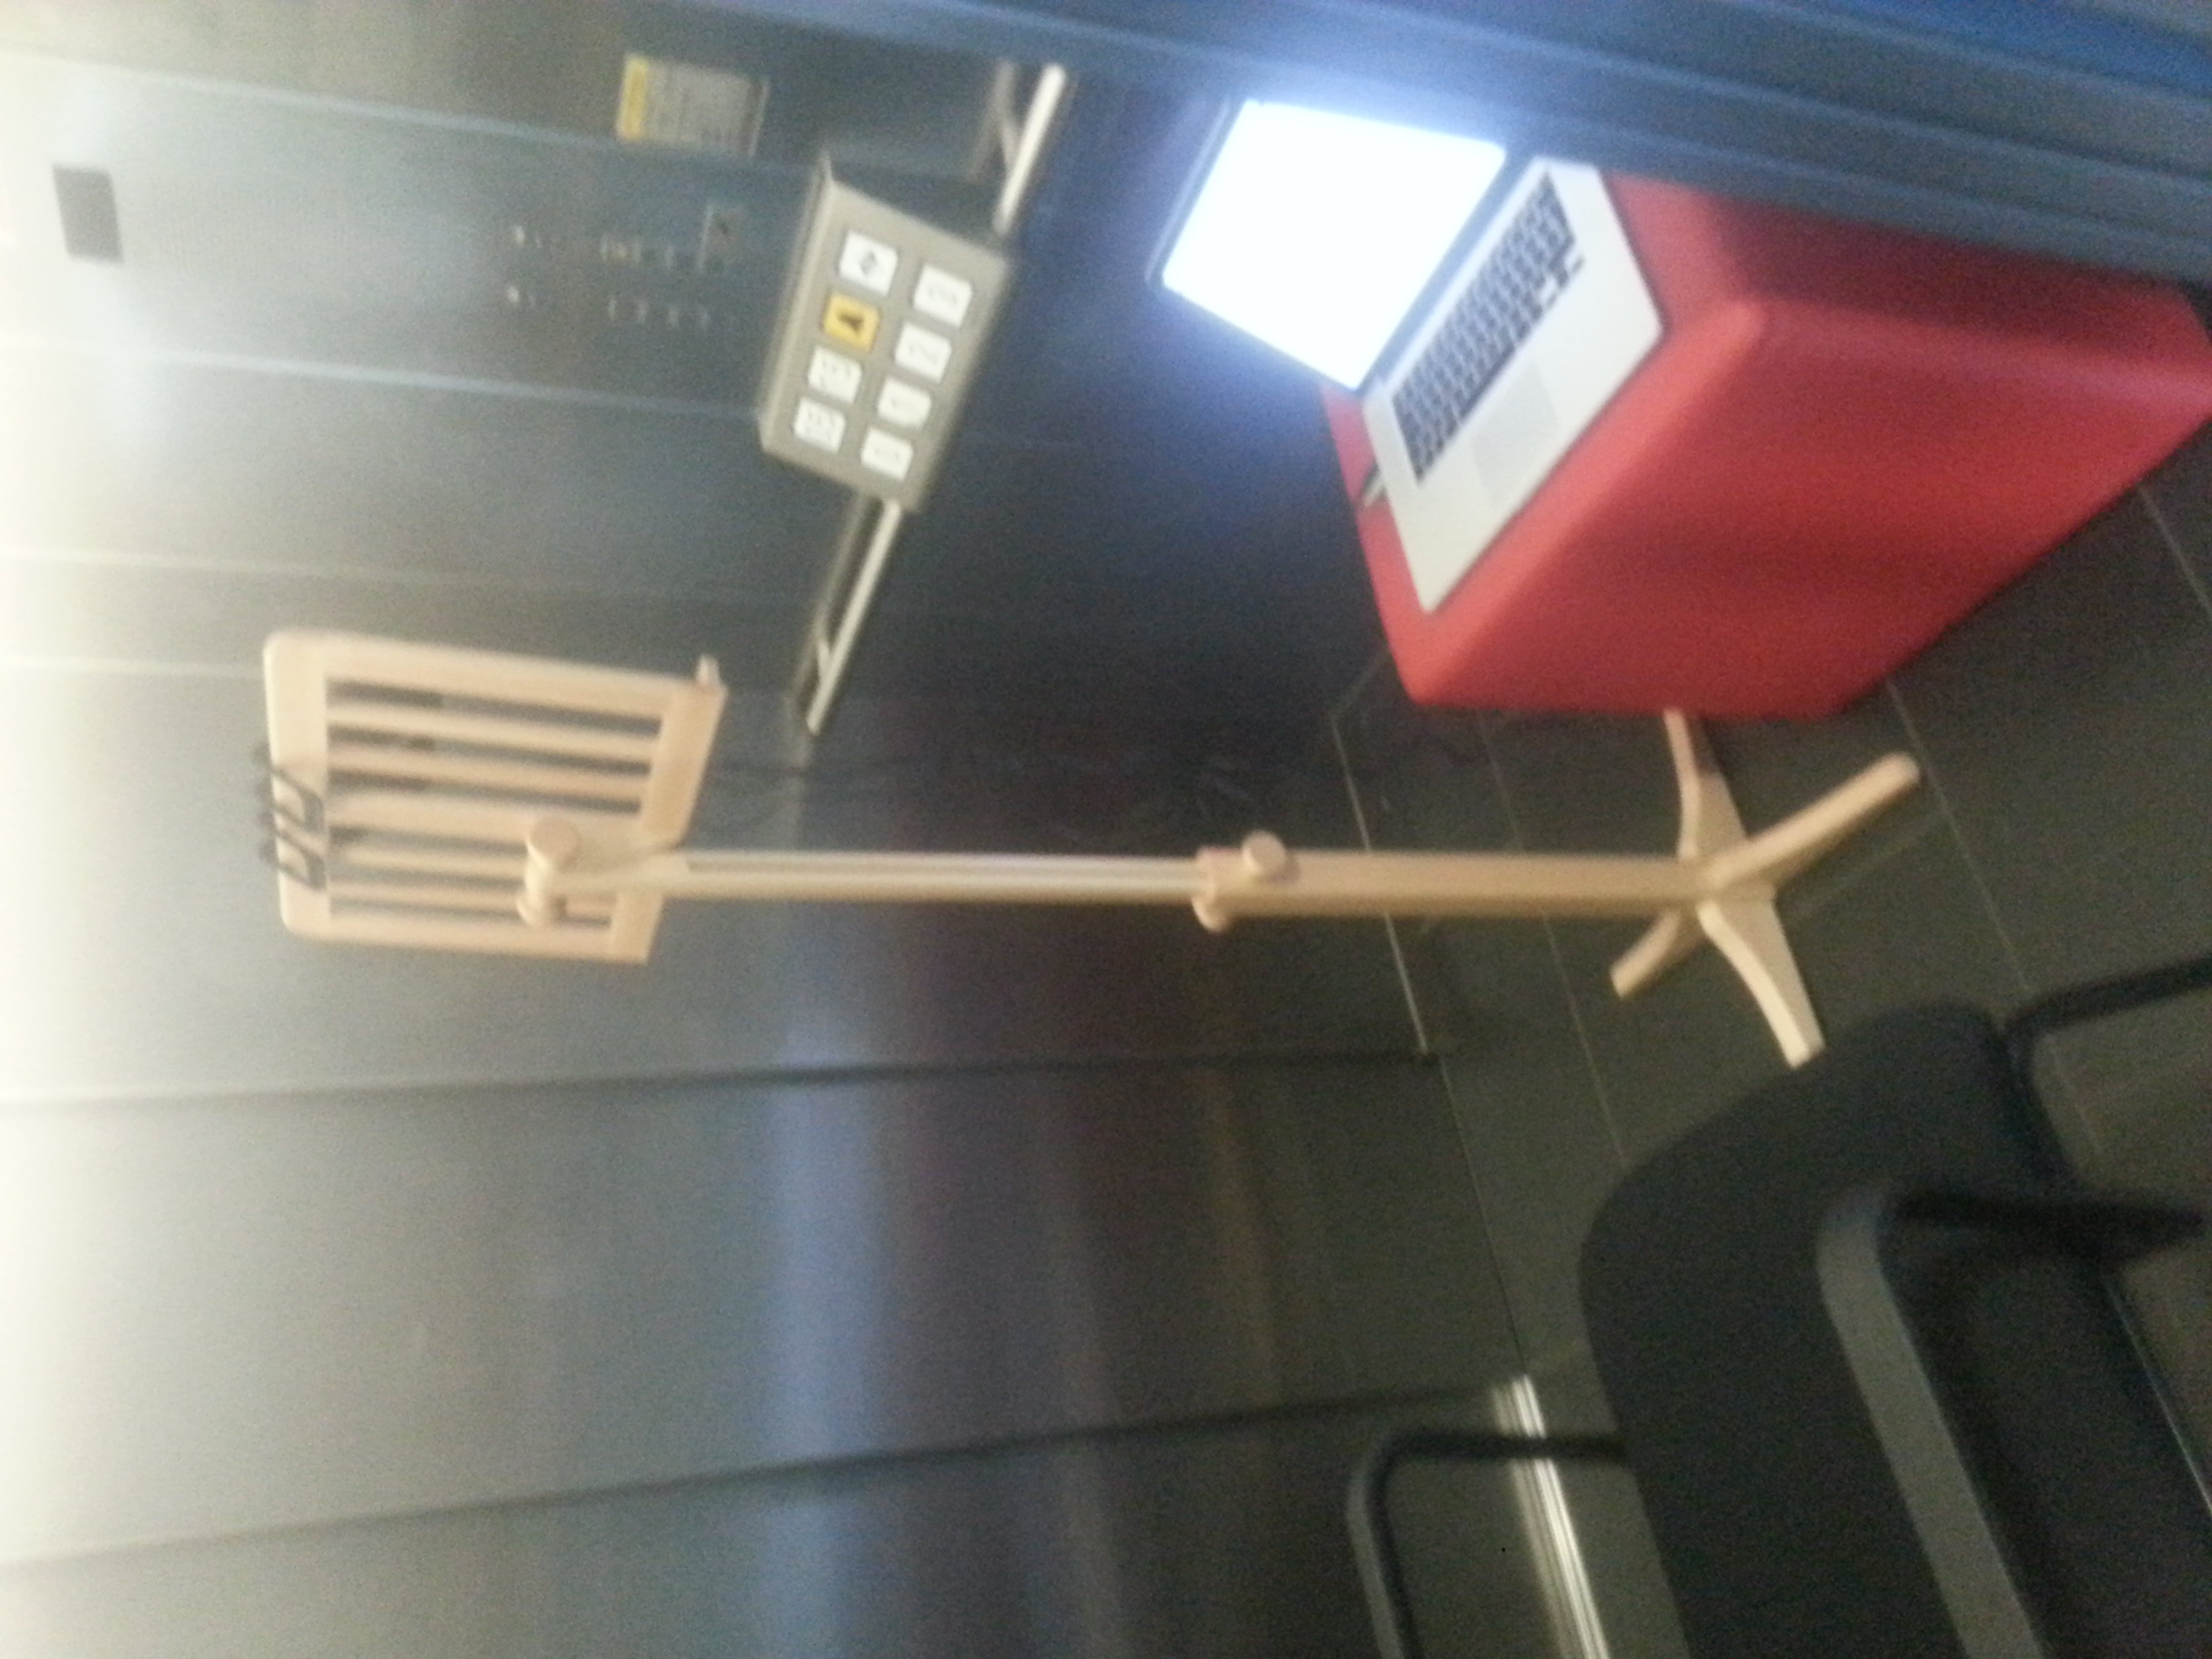
\includegraphics[scale=0.15]{setup_reverberation_rec.jpg}
\caption{Recordings setup.}
\label{fig:recordingsetup}
\end{figure}



\noindent To account for the noise of the elevator, its sound when moving, the sound of the doors opening and closing and the reverberation with open doors on the different floors and other noises from outside of the elevator, recordings were done via the elevator's built-in microphone. 
The setup used for this can be seen in picture \ref{fig:recordingsetup}.
It consisted of two loudspeakers positioned on a music stand at the height of approximately 150cm, at a distance of approximately 20cm from the elevator's microphone. 
The recordings made in the lab were played through the loudspeakers and recorded with Praat via the elevator's microphone. 
While the recordings were being played, the elevator was moved between the floors, its doors were opened and closed and kept with its doors opened and closed on different floors.


\subsubsection{Language model}

%\input{jsgf_summary.tex}
\subsection{General thoughts}
Before actually starting to work on the dialogue itself, we decided on how a dialogue with the EllaVator should look like. \\

We came up with the following model: \\


\begin{figure} [ht]
\center{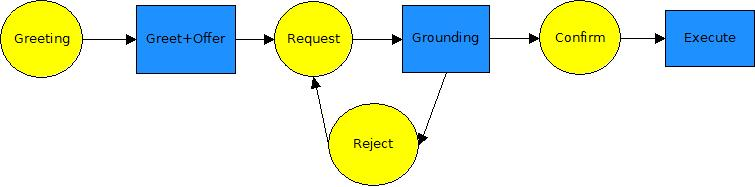
\includegraphics[scale=0.8, angle=0]{Dialogue_model.jpeg}}
\caption{A model for the Dialogue}
\label{fig: Dialogue flow}
\end{figure}

In the figure shown above commands from the user are marked in yellow, the answers from the EllaVator are marked in blue.
Here is a table giving example sentences for the states indicated by the figure above: \\


\begin{tabular}{|ll|}
\hline
Greeting & The user greets the Ellevator with a keyword \\
  & and thus activates the system.  \\
Greet + Offer & Hello, how can I help you? \\
Request & Take me to floor/room XY/ Name\_of\_a\_person \\
Grounding/Clarify & You'd like to be taken to ...?\\ 
 & I didn't get it, could you repeat that? \\
Confirm & Yes \\
Reject & No \\
Execute & Okay I shall now take you to ... \\ 
 & *here the elevator should also start the action of moving* \\
\hline 
\end{tabular}
\newline
Of course the actual system should be able to understand a variety of sentences and maybe alternate the answers but the dialogue itself can be kept as simple as it is shown in the graph.  \\

We thought about including some chatting with the user or small Easter eggs. 
We have therefore made measurements on how much time the average user spends in the elevator to determine how much time there is for the dialogue.
On average the elevator needed 40 seconds to go from the ground floor to the top and 21 seconds for going down. Opening the Doors takes 4 seconds, closing them 5.5 seconds.
With this in mind we decided to keep the dialogue as simple as possible as one of the reasons for everyone using the elevator is to be faster compared to taking the stairs and that maybe the likelihood of people using the speech interface would be lower if too much time was spend on such interactions.\\

Instead, we discussed whether we should enable the user to merge the state "Greet" with the state "Request" which would allow for the user to both activate the elevator and also enter where they would like to be taken to.
This would skip one state from the user as well as one step from the elevator.
Depending on the confidence of the user input we also considered leaving out the "Grounding" state to have a shorter dialogue.\\

In the end we implemented the system as was described in the graph above and decided that we should first try out how the system works on the real elevator before making further changes.\\

Another thought we had but have put aside to work on after we have seen our project running on the actual hardware was that it might be the case that more than one person enters the elevator and that these people might have different destinations.
Of course it would be possible to just run the dialogue with one person, take them to their destination and then run the dialogue again with the next person.
This approach might however be inconvenient. 
It might be more natural to enable the system to take more then one request.\\

Another problem that arose when thinking about the scenario of more than one person entering the elevator, was that they might not share the same language.
We decided to provide an English as well as a German version of our system.
So the problem was not only to allow for multiple inputs but also for multiple inputs in different languages.\\
\newline

\textbf{
\begin{center}Switching between languages... \\
\underline{Our thoughts on this are collected in ticket 80}\\
@Naska \\
@Laura \\
does one of you feel like writing a little about this issue?
\end{center}}
\subsection{Dialog-manager}

The dialog manager is responsible for keeping track of the conversation and deciding the next move of the system for each input. The domain of our project is fairly limited. Most conversational situations consist of the user naming a location and the machine taking the action of moving to that location and reassuring the user that it had understood the command. This can described by deterministic If...then... statements. A dialog manager that models the conversation flow as an deterministic FSA is well-suited for our needs.
When choosing the dialog manager for our project we considered the following factors: It had to be open source, preferably Java, well documented.
We were also looking for code that was actively maintained.
We reviewed a few potential contenders:
\begin{itemize}
\item[IrisTK] \hfill \\
TODO
\item[InproTK] \hfill \\
The most exciting asset of this dialog manager was incremental processing.
The code is well maintained and actively developed. 
However, we failed to build a demo that uses incremental features due to the lack of documentation so we dropped this option.
\item[OpenDial] \hfill \\
OpenDial is probably the most popular open source dialog manager.
After successfully implementing a short domain-relevant demo we opted for this manager.
For more detailed description of OpenDial see next section.

\end{itemize}
\subsubsection{Opendial}
\subsection{Dialog Manager - this small chapter has to be synchronized with the previous one - }

After a sound has been recognized as speech and the words have been extracted by the grammar, the system needs to decide which action to take and also perform it.
This process is done in the so called ”Dialog Manager”. When and how the system should react to speech is defined in this program.

For the speaking elevator ”EllaVator” the Dialog Manger ”Open Dial” was used.
Therefore I would like to give a quick introduction to the Dialog System Open Dial in the following Chapter.

\subsection{Open Dial}

Like most Dialogue Managers Open Dial also consist of three different components which interact to create a dialogue. 

The first component is responsible for the recognition of language. 
In Open Dial this component is called „ Natural Language Understanding model”. 
The output of the first process is passed on to the next component which checks if there was a instruction given which action should be  be performed upon that input. 
Such actions might be showing something on a GUI, starting a task or simply selecting an answer to the users input. 
In OpenDial this part is called „Dialog Manager”.
The third and last component is called „Natural Language Generation module” and is basically the opposite of the „Natural Language Understanding model”. 
The „Natural Language Generation model” Generates Language from the output of the „Dialog Manger”. 
Though the component is named ”Natural Language Generation model” the output of a Dialogue System is not necessarily speech, but the output is often designed so that it can be easily used to generate speech with a TTS. 
This is also the case for open Dial. 
Open Dial also offers a GUI where the dialogue (input, as well as output) is displayed without having to use further plug-ins.

\subsubsection{Domain}

All of the components mentioned above are located in the so called Domain file.
A dialogue designer working with Open Dial will in most cases just have to work on this one file. For easier readability, it can of course be split into smaller files, which will then have to be imported into one single file. \newline

In this file the users input will be first transformed into a XML structure and then further processed.
Some systems fill this structure with semantic information. 
OpenDial however basically passes variables through the components of the system. 
The dialogue designer can then assigns values to those variables which will ultimately determine the flow of the dialogue. 
There is a convention for the naming of the variables, they can however be named to the dialogue designers liking. 
As all information is being passed through variables the correct naming is important though. 
All three components have a slot ”trigger” at the very beginning of their structure. 
The value given to this slot has to be the name of all variables which are to activate this component.
For example giving the component this trigger: 
\textless model trigger=”a\_u” \textgreater will make it respond to all variables with the name ”a\_u”.  \newline

So the variables in Open Dial do not only carry the value through the system but their names also determinate which module should continue to process that variable. The most common way to link them was described above: Having the Natural Language Understanding module process the users input, the Dialogue Manager process that input and then responding using the Natural Language Generation module. 
In case there is no further processing needed one might also decide to directly link Natural Language Understanding module to Natural Language Generation module. 
If the System should maybe ask a question after having said something, it might also be possible that the dialogue designer might want to trigger the Natural Language Generation twice, either linking Natural Language Generation to Natural Language Generation module or Natural Language Generation module to the Dialogue Manager which again links back to the Natural Language Generation module. \newline

The domain-file is first subdivided into three parts as they each represent one components these parts are called modules. 
The modules themselves are again subdivided into rules. Every rule in this file represents one command. 

\subsubsection{Natural Language Understanding module}

The first model to receive input is the ”Natural Language Understanding module” (NLU). 
Depending whether further plug-ins are used this module will get its input either directly from the user or from the plug-in.
Open Dials NLU component is able to work with plain text input from the user, but in the case of the Ellavator project the User shall also be able to use speech commands to operate the elevator, therefore the NLU in this project receives input from the grammar file of the Sphinx plug-in.
The grammar of the Sphinx plug-in already does part of the work, which would be usually done by the NLU alone.
There is only a very limited amount of commands which the elevator is able to execute.
Each of those can be however be triggered by various expressions. As different people will use different words and structures to express themselves.
Therefore a domain-file that should be capable of doing something should have at least one rule which can be activated by at least one expression. \newline

In the example shown below there is a rule which models the command of changing a direction.
A rule consists of at least one case-expression.
A case-expression itself consists of a ”condition” and an ”effect”.
 In the ”condition”, as the name already states the Dialogue Designer can define under which circumstances a case-expression will match the users input.
These conditions are connected using a logical operator.
In most cases one would want to use the conditions ”or” as either one of those expressions should trigger the rule.
 The ”effect” will be the value passed on to the TM.
As stated before this is done by assigning a variable of the proper name a value.
In the case of the example below the variable is assigned the value of the function of changing to floor to the level of the given parameter. 
\newline


\textless rule \textgreater \newline
\indent \indent \textless  case \textgreater \newline
\indent \indent \indent \textless condition operator=”or”  \textgreater \newline\indent \indent \indent \indent \textless if var=”u\_u” value=”go to second floor” relation=”contains”/  \textgreater \newline
\indent \indent \indent \indent \textless if var=”u\_u” value=”take me up to the second floor” \newline
\indent \indent \indent \indent relation=”contains”/ \textgreater \newline
\indent  \indent \indent \indent \textless if var=”u\_u” value=”second floor” relation=”contains”/ \textgreater \newline
\indent \indent \indent \textless /condition \textgreater \newline
\indent \indent \indent \textless effect prob=”1” \textgreater \textless set var=”a\_u” value=”Request(second)” / \textgreater \newline
\indent \indent \indent \textless /effect \textgreater \newline
\indent \indent \textless /case \textgreater \newline
\indent \indent \textless case \textgreater \newline
\indent \indent \indent \textless condition operator=”or” \textgreater \newline
\indent \indent \indent \indent \textless if var=”u\_u” value=”go to thrid floor” relation=”contains”/ \textgreater \newline
\indent \indent \indent \indent \textless if var=”u\_u” value=”take me up to the third floor” relation=”contains”/ \textgreater \newline
\indent \indent \indent \indent \textless if var=”u\_u” value=”third floor” relation=”contains”/ \textgreater \newline
 \indent \indent \indent \textless /condition \textgreater \newline
\indent \indent  \textless effect prob=”1” \textgreater \textless set var=”a\_u” value=”Request(third)” / \textgreater \newline
\indent \indent  \textless /effect \textgreater \newline
\indent \indent \textless /case \textgreater \newline
\indent \textless /rule \textgreater \newline


In the example above one rule is shown.
This one rule includes two different commands.
They are gathered in one rule as the both are orders to switch a floor.
The only difference is the floor level they have.
Resulting in different parameters which are given to the function of the variable ”a\_u” in the ”effect” slot. \newline



As stated before every user will use different words to express themselves.
To cover up all possible utterances for a command is impossible.
But one should try to at least cover the most common ones,  to make the dialogue more natural for the user.
This part can also be done in the grammar of Sphinx.
Open Dial offers a few possibilities to do so.
The first possibility would be to simply list all the expressions as it is shown in the figure above.
But as can be easily seen in the example above, there is only a small difference between the sentences.
If one would like to cover all possible sentences by merely enlisting them the Domain file will not only get extremely huge it will also be hard to read.
Therefore it is recommended to use the following expressions which will help to keep the Domain file smaller and easier to read which will make it less prone to mistakes and errors if used in the right amount. \newline


\begin{tabular}{|ll|}
\hline
	a? & The word „a” may or may not occure in the expression .  \\
\hline
	(a \textbar b \textbar... \textbar x) & One of the symboles written	in the brakets has to occure.\\
\hline
	(a \textbar b \textbar... \textbar x))? & One of the symboles written in the brakets may or may not occure.  \\
\hline
\end{tabular}
\newline

This table shows the expressions which can be used to structure a the NLU. \newline \newline

In the example used above all three user-utterances could be shortened down using the expression:
\textless if var=”u\_u” value=”(go \textbar take me) (up to the)?  second floor” relation=”contains”/ \textgreater

Using this expressions is therefore recommended.

\subsubsection{Dialogue Manager}

If the variable which was assigned in the NLU module was named correctly it should, in most cases, first be passed trough the Dialogue Manager (DM).
In the Dialogue Manager the effect of a rule is triggered. A mapping occurs which links the input provided by the NLU to another structure that will trigger a reaction of the system.
As was said in the last subchapter, values in Open Dial are saved within and passed trough variables, the input from the NLU will therefore be assigned to another variable. \newline
Just like all other modules each command in the DM is divided into rules, each of them having a condition, when they are to be activated. 
Therefore in this component the output of the NLU component will be matched against all conditions in the DM. 
As soon as one matching rule is found, that rule is triggered which sends the ”effect” of that rule.
The effect of a rule is saved into a variable.
If no further work, like printing information on a GUI is done, one could argue, that all the DM does is basically linking two variables, the one given in the ”condition” to the variable written in the ”effect”.
Of course not all parameters do have to be listed.
It is sufficient to merely put a placeholder in curly brackets to indicate that there is a parameter to be passed on. \newline


\textless rule id=”Movement” \textgreater \newline
 \indent \indent \textless case \textgreater \newline
\indent \indent \indent \textless condition \textgreater \newline
\indent \indent \indent \indent \textless if var=”a\_u” value=”Request(\{x\})” / \textgreater \newline
 \indent \indent \indent \textless /condition \textgreater \newline
 \indent \indent \indent \textless effect util=”1” \textgreater \newline 
 \indent \indent \indent \indent \textless set var=”a\_m” value=”floor(\{x\})” / \textgreater \newline
 \indent \indent \indent \textless /effect \textgreater \newline
\indent \indent \textless /case \textgreater \newline
\indent \textless /rule \textgreater \newline

The figure above shows  a rule called ”Movement” which links the users input ”Request” with any parameter to the effect of that input.
The variable with the name ”a\_m” and the value ”floor” with the input of the Request is send.
The parameter specified in the placeholder ”x” written in curly brackets.

\subsubsection{Natural Language Generation module}

The last part of the system generates the speech. 
Without any further plug-ins this will be done by printing the text to the GUI.
As stated before, this component basically does the opposite of the Natural Language Understanding module. 
Instead of transforming the users input into an XML structure, the system takes the last components output, which is a variable embedded in an XML structure and transforms it back to plan text, either spoken if plug-ins are used or printed on the GUI, if no plug-ins are used. \newline

Each command is again given its own ”rule” and ”case” structure, in which ”condition and effect are included. 
The effect of this rule is saved in a variable but also used as output for speech. \newline

\textless rule \textgreater \newline
\indent \indent \textless case \textgreater \newline
\indent \indent \indent \textless condition \textgreater \newline 
\indent \indent \indent \indent \textless if var=”a\_m” value=”floor(\{x\})” / \textgreater \newline
\indent \indent \indent \textless /condition \textgreater \newline
\indent \indent \indent \textless effect util=”1” \textgreater \newline 
\indent \indent \indent \indent \textless set var=”u\_m” value=”Okay, I will now take you to the {x} floor.” / \textgreater \newline
\indent \indent \indent \textless /effect \textgreater \newline
\indent \indent\textless /case \textgreater \newline
\indent \textless /rule \textgreater \newline

The example above shows one rule from an NLG module. 
In this rule a variable to which a function  is assigned, triggers the speech output of an acknowledgement from the system.


\subsubsection{some Other}

\subsection{Text-To-Speech System Mary}
The final step in creating the speaking elevator "Ella" was of course to make it actually talk to the user.
For this a Text-to-Speech system (TTS) had to be used. A text to speech system will read out information to the user, transforming written into spoken text.
Such programs are wildly used today. 
There are announcements at the train station informing guests about delays or if there are changes causing a train to depart from a different platform as planned.
There are screenreaders for the visual impaired, which read out the elements of a screen, as well as systems which are used by the speech impaired to communicate and speak in their stead.
One of the most famous talking applications is the Dialoguesystem "Siri" (Siri inc) which is used since 2011 on the iPhone. \newline \newline
For our talking elevator we wanted to use an open source TTS. 
We did choose the system Mary for this task.
Not only was it developed in cooperation with the university of Saabrücken, it also offers many advantages to other TTS and therefore seemed perfect for the task.\newline

Written in the programming language Java it was designed in a collaboration between the  "Language Technology Lab" of the DFKI \footnote {(\textbf{D}eutsches-\textbf{F}orschungszentrum für \textbf{K}ünstliche \textbf{I}ntelligenz) - The German Research Centre for Artificial Intelligence} and the faculty for phonetics of the university of Saarbrücken.
As Mary is an open Source project one can not only see the code but is also allowed to change and adjust it to ones needs.\newline \newline
The name Mary is an acronym for \newline 
\begin{center}"\textbf{M}odular \textbf{A}rchitecture for \textbf{R}easearch on speech s\textbf{Y}nthesis".\end{center}
This name already states various facts about the system. 
It is build in a "modular architecture" which means that it consists of different components, each dealing with a specific task. We will take a closer look at these in the following subchapter.
The second part of the name states the purpose Mary was developed for.
It was developed for research having a modular structure and also being a open source project makes it really easy to use Mary for any research projects on speech synthesis. \newline \newline
Mary is a multilingual TSS, featuring the languages English (British as well as American), German, Telugu, Turkish, Russian, Swedish and Italian. 
Further languages might be included in the future, but can also be added by any user. \newline \newline
The following information about the structure and components of Mary is taken from the paper: 
The German Text-to-Speech Synthesis System MARY:
A Tool for Research, Development and Teaching by Marc Schröder Marc and Jürgen Trouvain.

\subsubsection {Modules}

Mary is subdivided into different modules. 
This allows the used to take a look at the output of each of those components. 
One could also interchange small details on one component and observe the output on the complete system as well as completely interchanging a component.

\subsubsection* {Input}

Mary acepts differnt kind of inputs, the simplest one being plain text. 
But also Mark-up Languages such as SABLE or SSML can be used. 
These are based on the Mark-up Language XML and are developed especially for the use in TTS.

In case of the elevator we only pass the output of the Open Dail Dialogue Manager to Mary, which is plain text.
Any input given to Mary will be transformed into a "MaryXML Mark-up Skeleton". 
A skeleton which already has different slots which will be filled by the system in the other modules.
If the input was already in a form of Mark-up language the keys assigned in this Mark-up Language will be kept and added to the Skeleton some of the values however might be dropped.

\subsubsection* {Tokenizer}

The tokenizer identifies the tokens of a text. The output of this module will be sentences and words which will be marked as such.
Any token will be enclosed by "\textless t\textgreater ...\textless  t\textgreater". 
These marks are however just placeholder. 
Later on, further information will be saved in these slots.
Analogous a sentence is enclosed by "\textless s\textgreater ... \textless s\textgreater". 
Marking a dot as a sentence might seem obvious at first, but can prove quite difficult if there are other tokens in the text which also come with a dot, but do not mark the end of a sentence, such as the dot placed after titles.

\subsubsection* {Preprocessing}

This module also called "Text-normalisation" does only work on very specific tokens.
It is only needed for acronyms or numbers.
For acronyms the system will have to decide whether to pronounce them as one word or spell each letter out separately.
Numbers are divided into ordinal- and cardinal numbers.

\subsubsection* {Tagger and Chunker}

This module has two different tasks to solve. 
The Chunker labels the constituents in each sentence.
These are distinguished between adjective-, nominal- and prepositionalphrase. "Chunkie" is used for this task. 
It was developed by Skut and Brants in 1998. 
"TnT", the tagger used was also developed by Brants in 2000. 
It is a statistical POS-tagger working with trigram provabilities \footnote {To assign the correct word class the tagger does not only consider the current word but also the two words which were used last, making it a total of three words.} in order to assign every word its proper word class.
The wordclasses are provided by the Stuttgard-Tuebinger-Tagset (Schiller et. al., 1997)

The findings of the two components are saved within the placeholders that were created by the tokenizer.
Unfortunately this also means that some of the information given by the Chunker will be lost. This would be the case for local ambiguities.


\subsubsection* {Phonemisation}

This module also describes the work of several smaller steps.
The output of this system will be the transcription of every word into phonetic transcription.
To able to do this however there still needs to be some information extracted.
One of the steps needed is called "inflection endings". 
In this process the tokens marked in the step "Preprocessing" are reviewed.
With the information given by the Chunker in the earlier steps as well as under the use of the morphologic analyser "Mmorph" (Petitpierre and Russle, 1995) these tokens such as ordinal number can now be expanded.\newline 
In this step Mary will also check its a dictionary specifically designed for Mary by the DFKI.
It contains information about the stem of a word as well grammatical information, which reduces the amount of data as regular words can be conjugated and inflected according to those rules.
The lexicon also covers many of the acronyms. 
It can even handle composed words quite will, which is especially important for the German language. \newline 
In case there is no information found about a word in the dictionary the "letter to sound conversion" will be used.
Of course this module can not know whether a word unknown to the system is a acronym or an actual word. 
This problem was solved rather simply. 
All words which have less than five letter will be treated as acronyms and each letter will be pronounced separately. 
In case the word is longer it will be read out as a complete word.
The "letter to sound conversion" (Alan Black et al., 1998) was trained on the dictionary to obtain about how to pronounce a word.
The decomposition was trained statistically on the database CELEX (Baayen et al. 1995).
After decomposing every word they will be matched against a list containing morphemes which change the intonation of a word.
The remaining morphemes are processed according to language specific rules.
Hyphenation will also be defined by phonological principals such as the sonoraty hierarchy of phonemes \footnote {Schröder, Marc, and Trouvain Juergen. "The German text-to-speech synthesis system MARY: A tool for research, development and teaching." International Journal of Speech Technology 6.4 (2003): 365-377.} \newline
After these analysis an algorithm decides which syllable will get the main stress.\newline
The output of this module only contains the SAMPA transcription and a note in case a word was processed by the "Letter to sound conversion". 
Information on intonation will not be seen in the output.

\subsubsection* {Prosody rules}

After the last module has assessed the intonation of a word, this module will analyse the prosody of the entire text.
The end of a sentence is a classic example for the intonation of a sentence, but one of the most important aspect of prosody of a text are the pauses which have to be added to it.
These will be included by the program GToBI (Grice et al., 2002). 
With the aid of GToBI Mary distinguishes between six types of pauses, all being different in their length.
A pause for the end of a paragraph for example will be given the number 6, which is the longest pause there is in Mary.

Again the work of the chunker and tagger is of great importance for this module.
The output of the chunker will provide information on the structure of the sentence, for example whether a part of a sentence is a \emph{Vorfeld}. \footnote {Marc Schroder and Juergen Trouvain, 2003}
Though not all of the information will be seen in the output of this module, every word will contain a new field called "accent" in its placeholder, where the information about the intonation of the word will be stored.

\subsubsection* {Postlexical and Phonological process}

In this step the data will be revised and everything will be put into context.
Smaller details such as glottal stops or elisions at the end of a word are being added. 
After this step the skeleton which has been created at the beginning of the process is filled with the maximum of information being available to Mary.

\subsubsection* {Calculation of acoustic parameters} 

This module will abandon the structure of the MaryXML structure.
Instead the output will be a list of segments, their duration and the corresponding F0 value \footnote {The F0 value is a number describing the format 0, or the fundamental frequency of a voice and indicates the pitch.}
"The duration rules" by Brinckmann and Trouvain (2002) were used for this. These were created as an adaptation of the  "Klatt-Rules" (Klatt 1979; Allen et al., 1987) and define how long a tone will be.
The realisation is taken from GtoBI which was used to determine the pauses between the words in the earlier steps.

\subsubsection* {Synthesis}
In this final step the values acquired in earlier steps will at last be converted into sound.
The modular architecture of Mary makes it easy to interchange the synthesis module as long as it supports the format of the output given by the previous module.
Currently MBROLA (Dutroit et al., 1996) is used in by Mary, which was selected as it creates a low distortion in the signal.
\section{Implementation details}
\subsection{Raspberry pi}
pi4j
\subsubsection{Raspberry Pi Virtualization}
By setting up a virtual Raspberry Pi, we can further test our software without physically accessing the Raspberry Pi and burning disk images all the time, even after all automatic tests are passed.

Raspberry Pi uses an ARM processor, so the only tool available to emulate it on PCs is \texttt{qemu}.

Basically we follow the instructions from \url{http://www.linux-mitterteich.de/fileadmin/datafile/papers/2013/qemu_raspiemu_lug_18_sep_2013.pdf} but use the latest Raspbian image instead, which can be downloaded from \url{https://www.raspberrypi.org/downloads/}.

And download \texttt{kernel-qemu} from \url{http://web.archive.org/web/20150214035104/http://www.xecdesign.com/downloads/linux-qemu/kernel-qemu} because the original page is unavailable.

Currently this solution has several drawbacks, mostly notable ones are low speed and lack of serial port support.

\vspace{\baselineskip}

Note:

\begin{itemize}
\item The second line of \texttt{/etc/udev/rules.d/90-qemu.rules} is indeed \texttt{KERNEL=="sda?", SYMLINK+="mmcblk0p\%n",}, there is a typo in the picture.
\item Although the new RPi 2 model has an ARMv7 processor, Raspbian is still compiled into ARMv6 (for compatibility with old models), so emulating with \texttt{-cpu arm1176} is reasonable.
\end{itemize}
\subsection{Serial control of elevator}
\subsection{Testing}
\subsection{Development tools}

\subsubsection{Gradle}
Gradle\footnote{http://gradle.org/} is a build automation tool and simplifies the build process drastically.
Instead of having a readme file that explains how to build the project, building the project is as easy as executing \texttt{./gradlew build} on the command line.

Gradle is configured in the file \texttt{build.gradle}.
Although it looks like a configuration file, it is actually fully functional code written in Groovy\footnote{http://www.groovy-lang.org/}, a programming language based on Java.

We included a Gradle wrapper in the repository.
This file called \texttt{gradlew} (and \texttt{gradle.bat} for windows) download and run the right Gradle version when executed.
It is recommended to use this file instead of using this file instead of any other locally installed Gradle, because it might be another version of Gradle.

The file \texttt{settings.gradle} specifies the gradle project structure by declaring several subprojects.
There is the opendial subproject, which is a copy of the dialog manager OpenDial\footnote{http://www.opendial-toolkit.net/}.
Next we have the pi4j subproject, which is a copy of Pi4j\footnote{http://pi4j.com/}.
We use it for serial port communication.
Next we have the sphinx4 subproject, consisting of sphinx4-core and sphinx4-data, which is a copy of the speech recognition software Sphinx4\footnote{https://github.com/cmusphinx/sphinx4}.
These subprojects are all forked on github from the originals, eventually adapted for our purposes and then included as a Git submodule.
Finally we have a subproject called prompts, that is our own making.
It contains example audio prompts for our application, that are used for the acoustic model training and for testing.

\subsubsection{github}
GitHub is a web platform for collaboration using git, which is a version control system. 
We used this system to allow several people work on the same project at the same time without overwriting each others changes.

For some of our dependencies (Sphinx, pi4j, OpenDial) we used git submodules to include them into our project. 
This gave us the possibility to adapt the original code for our purposes if necessary.
In order to download these dependencies when you clone the repository, you must therefore execute
\begin{lstlisting}[language=bash]
git clone https://github.com/EllaVator/EllaVator.git --recursive
\end{lstlisting}
or init and update all of the subprojects individually.

\subsubsection{Travis}
\subsection{Continuous integration with Travis CI}

Continuous integration is based on the idea that all developers send their changes to a common code repository as soon as possible, as we did on GitHub. 
Additionally these changes should be tested before they are merged into the main code repository. 
In order to do this automatically, it is necessary to automate the build process completely, as we did using Gradle.
If the build succeeds, all unit and integration tests can be executed, which prevents non-working code to enter the main repository if the error is covered by a test case.
This procedure is much better than having each developer running the tests before committing the changes to the main repository for a couple of reasons.
Firstly it does not rely on the developer to run all the tests which can be easily forgotten or skipped because the developer does not see the whole effect his modification has.
Secondly the project is built in a “neutral” environment that should be a close copy of the production environment if possible. 
This way for example code that runs fine on the developer's Windows machine but not on Linux can be detected.

As it integrates seamlessly into GitHub, we decided to use Travis CI as our continuous integration service. Each pull request gets marked by colors: yellow means the build is still running, red means failed build or failed test, green says everything is OK. In each pull request there is a link to Travis that gives details about the build process, too.

Travis is configured by a file named \texttt{.travis.yml} in the root directory of the project. 
It is not even necessary to specify that the build process is handled by Gradle.
Travis can detect this automatically, given that we specify groovy as our project language (\texttt{language: groovy}).
We needed to use Java 8 because this is a minimum requirement for Opendial.
Also, Travis must install the \texttt{sox} command, which is used to extract single sentences from our test audio files in the prompts subproject.
Finally, we cache the gradle files to speed up the build process (otherwise the Gradle wrapper will download Gradle every time).

Each developer can add Travis to his own repositories, too.
That way failures can be detected even before sending a pull request.
Travis can be activated by signing up on \url{https://travis-ci.org/} using your GitHub account.
Then go to your profile page on Travis and activate the GitHub repositories you want to be watched (which must contain a \texttt{.travis.yml} file).
From then on every push to these repositories will trigger Travis to build and run tests and send an email about the result.



\include{bibliography}

\end{document}
